% \documentclass[12pt]{article}

%%v helpful MIT exam schema, see http://www-math.mit.edu/~psh/exam/examdoc.pdf
 \documentclass[9pt]{exam} 
% \qformat{\textbf{Question \thequestion}\quad \thepoints\hfill } % Large depth to make space}
 \renewcommand{\thesubpart}{(\roman{subpart})}
 \renewcommand{\subpartlabel}{\thesubpart}
 \footer{}{}{Page \thepage\ de \numpages}
\addpoints
% \pointsinmargin
% \boxedpoints
%\renewcommand{\questionshook}{\setlength{\itemsep}{1cm}}
%\renewcommand{\partshook}{
%	\setlength{\itemsep}{0.5cm}
%    	\setlength{\leftmargin}{-10pt}%
%}

\usepackage{cmbright}

\pagestyle{empty} %for handouts
\addtolength{\jot}{2em} % this makes all formulae a bit more spaced vertically for handouts
\setlength{\parindent}{0pt} %we're not writing a novel
%\renewcommand{\arraystretch}{2} %makes tables taller, so easier to write in

\usepackage[fleqn]{amsmath}
\usepackage{amssymb} %standard classy maths symbols
\usepackage[a4paper, margin=1in]{geometry} %makes it easy to specify where to put stuff on the page

\usepackage{siunitx} %v handy way of getting SI units to typeset correctly...
\sisetup{locale = FR} %... and now it will use a comma for decimals

\usepackage[utf8]{inputenc}

% \usepackage[french]{babel} % frenchify everything (e.g. a Table becomes a Tableau)
\usepackage{lmodern} % font with nicer French characters than standard
\usepackage{textcomp} % and more help for special characters

\usepackage{tcolorbox} % basic but good package for boxes around text
\tcbset{colback=black!5!white}
\usepackage{color} % colours
%\newcommand{\fillin}{\color{black!1!white}} %makes the text disappear
%\definecolor{fillin}{rgb} {1.00,1.00,1.00}
%\renewcommand{\fillin}{\color{blue}} \definecolor{fillin}{rgb} {0.00,0.00,1.00} %makes the filling in text appear (in blue)

\usepackage{enumitem} % can change the labels on lists, items, enumerates

\usepackage{tikz, pgfplots} % interval diagrams, sets, etc.
\usetikzlibrary{calc,trees,positioning,arrows,fit,shapes}

\begin{document}
\sffamily

\textbf{Name:} \dotfill

\

\begin{questions}

\question[3] Calculate the midpoint $M$ of $A(-6;3)$ and $B(-2;5)$.
\\
\emph{Points for the formula, substitution of values, and the result}
\fillwithdottedlines{28mm}

\question[3] Determine the gradient-intercept form of the line $l$ passing through $M$ with gradient $-\tfrac{1}{2}$.
\fillwithdottedlines{35mm}

\question[2] $M$ lies on $l$. Calculate two other points belonging to $l$.
\fillwithdottedlines{21mm}

\question[4] Plot all the objects studied on these axes.

\begin{center}
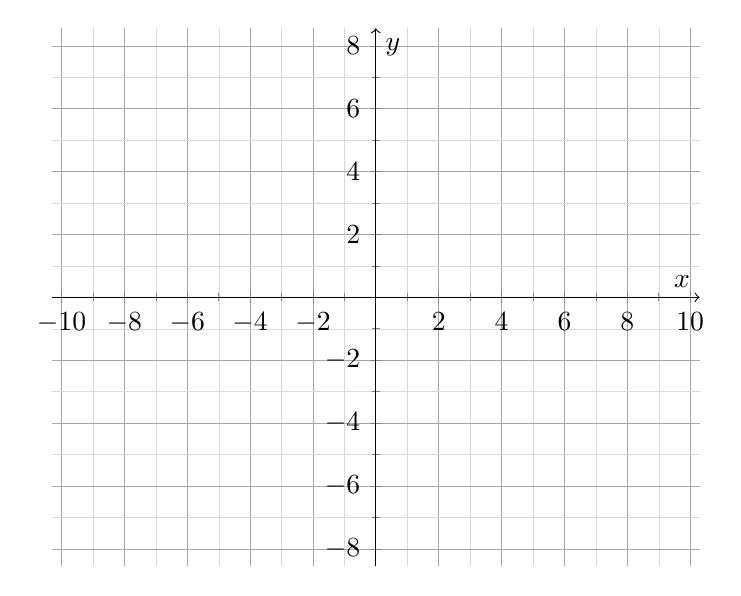
\begin{tikzpicture}
\begin{axis}[
	axis x line=middle,    % put the x axis in the middle
	axis y line=middle,    % put the y axis in the middle
	axis line style={->}, % arrows on the axis
	xlabel={$x$},          % default put x on x-axis
	ylabel={$y$},          % default put y on y-axis
	scale=1.2,xmin=-10.3,xmax=10.3,ymin=-3.3,ymax=3.3, 
	minor tick num=1,  
	grid style={line width=.1pt, draw=gray!30},
	major grid style={line width=.2pt,draw=gray!70},
	grid=both, ticks=both, axis equal=true]

\end{axis}
\end{tikzpicture}
\end{center}

\question \textbf{Bonus.} Calculate the distance from $B$ to $l$. \hfill \emph{Work overleaf.}

\end{questions}

\begin{tcolorbox}

\textbf{Name of marker:}

\begin{center}
\gradetable[h][questions]
\end{center}

\end{tcolorbox}


\end{document}